% Metoddelen redogör för vad du gjort och hur du gått tillväga; det är
% en beskrivning av den metod som ligger till grund för det du kommit
% fram till och hävdar i din rapport.

% Beskrivningen i metoddelen ska vara koncis snarare än helt
% uttömmande men ska samtidigt göra det möjligt att upprepa studien

% Metoddelen ska inte vara en omgjord labbinstruktion och den ska inte
% heller innehålla teori med mindre än att teoretiska hänsyn har haft
% en direkt inverkan på metoden.

% Metoddelen skrivs nästan alltid i dåtid (imperfekt) och ofta används
% passiv form för att beskriva forskningsaktiviteter.

\chapter{Metod}

\begin{draft}

Projektets genomförande bestod till störst del av konstruktionen av själva
läromaterialet, och där ingick skapandet av domänspecifika språk, skapandet av
den tillhörande lärotexten och publiceringen av denna på en hemsida. Därefter
följde en mindre del av utvärdering av materialet med en testgrupp som fick
svara på vad de tyckte om läromaterialet.

Det har inte funnits någon betydelsefull kronologi i projektet. I vilken ordningen aktiviteterna genomfördes spelar ingen roll för att förstå vad som genomfördes och hur det genomfördes. Resterande av kapitlet beskriver därför enbart aktiviteterna i sig, och inte i vilken ordningen de gjordes i relation till varandra. Självklart finns viss betydelsefull kronologi. Till exempel var (en del av) läromaterialet varit tvunget att vara skapat innan det kunde utvärderas, men sådana praktiska detaljer är obetydelsefulla för förståelsen.

\section{Konstruktion av läromaterialet}

Läromaterialet består av ett antal kapitel som vardera behandlar separata
områden. Skapandet av varje kapitel skedde därför till största delen fristående
från andra kapitel. Skapandet av kapitlena bestod i sin tur av tre faser,
som såg likadana ut för alla kapitel. Dessa faser var sökande efter område,
implementation av domänspecifika språk för området samt skrivande av lärotext.

Denna skapandeprocess kan delas upp i en graf med två axlar: en utefter kapitel och en
utefter fas. Det här illustreras i figur~\ref{fig:oversiktA}. Figuren visar att
varje kombination av kapitel och fas är en del i projektet som arbetades med.

\begin{figure}[tph]
    \centering
    \begin{subfigure}[t]{0.5\textwidth}
        \centering
        \frame{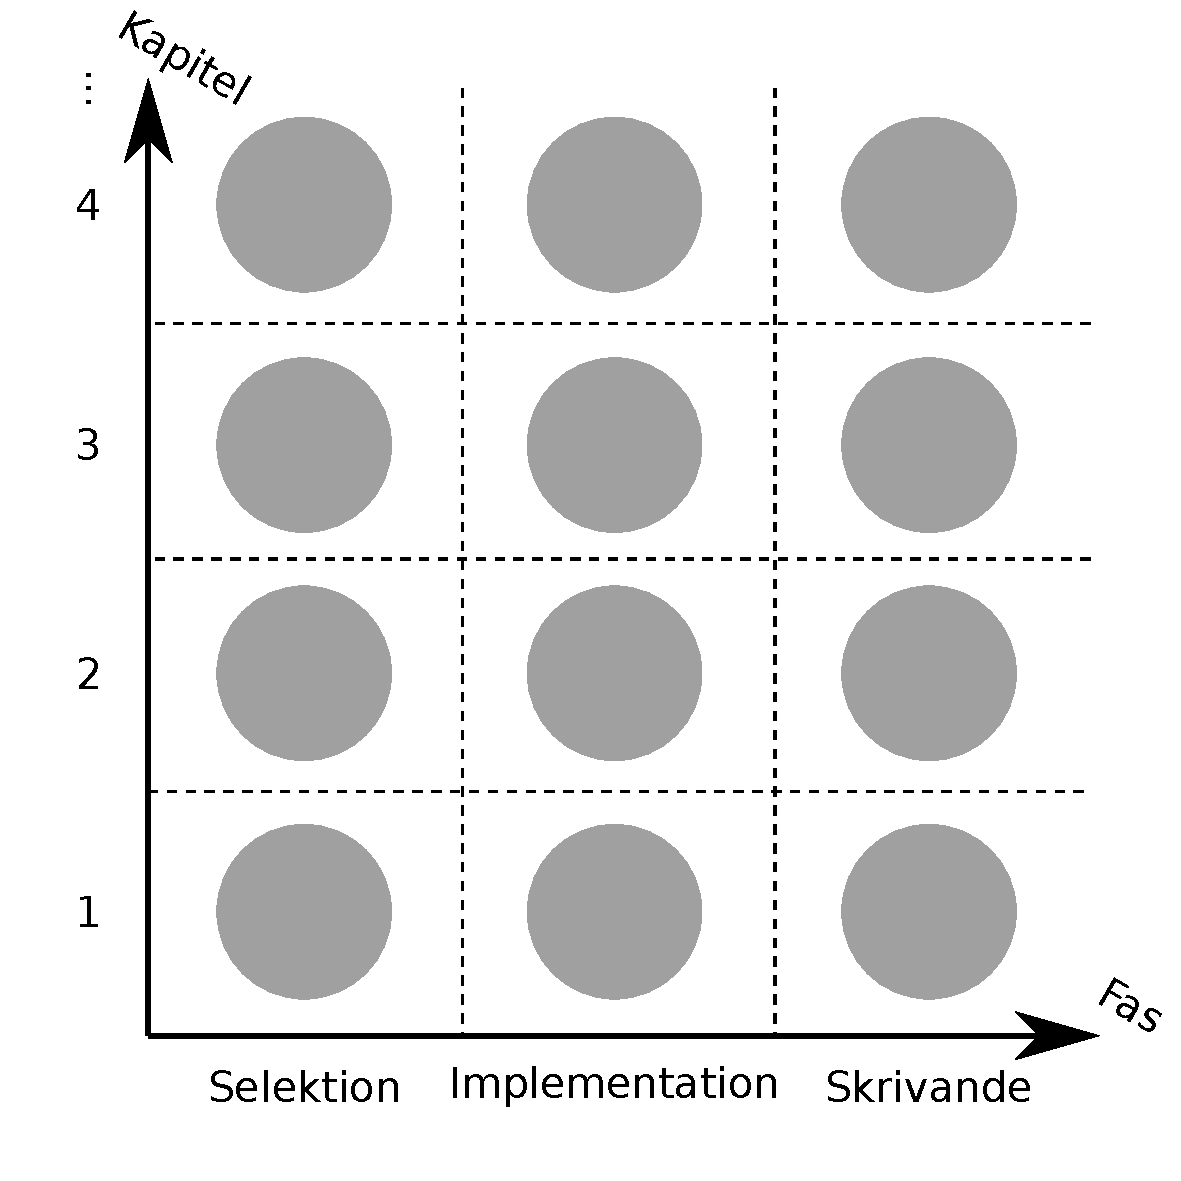
\includegraphics[width=0.9\linewidth]{figure/oversiktA.pdf}}
        \caption{Delarna visas distinkta och var för sig.}\label{fig:oversiktA}
    \end{subfigure}% <- This comment makes the figure lie side by side ¯\(°_o)/¯
    ~~~
    \begin{subfigure}[t]{0.5\textwidth}
        \centering
        \frame{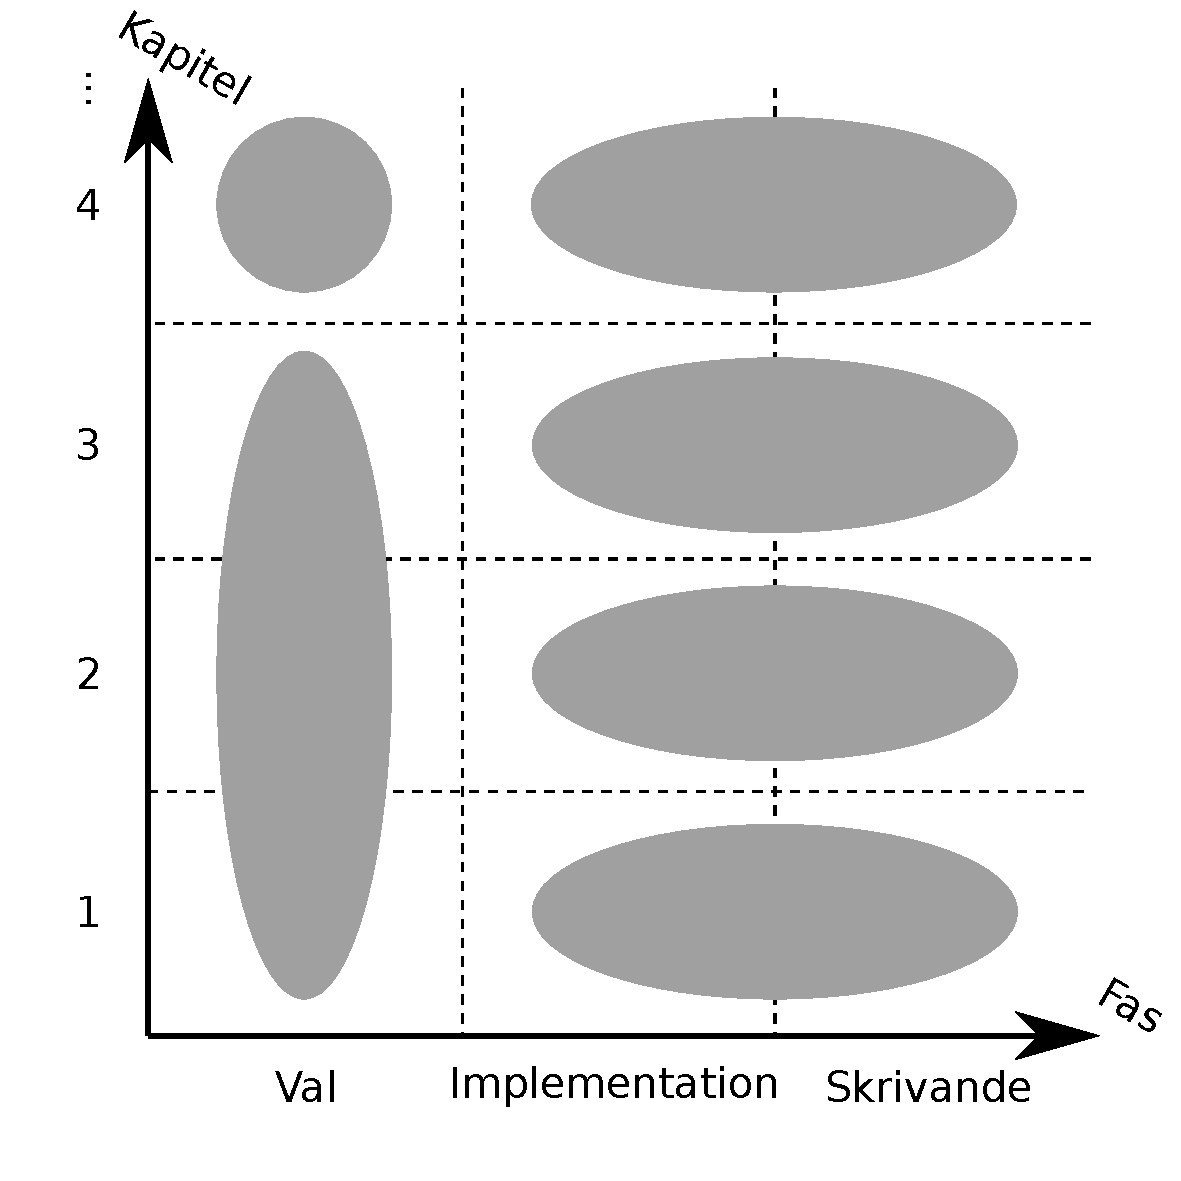
\includegraphics[width=0.9\linewidth]{figure/oversiktB.pdf}}
        \caption{Delarna visas med gränsöverskridande överlapp. Notera att
        implementation och skrivande \textit{alltid} var överlappande medan
      sökande \textit{ofta men inte alltid} var det.}~\label{fig:oversiktB}
    \end{subfigure}
    \caption{Översikt över hur skapandeprocessen av läromaterialet såg ut.
  Processen delas upp utefter två axlar: kapitel och fas. Varje kombination
  är en del som arbetats med och är gråmarkerad.} \end{figure}

Även om detta sätt att dela upp processen är översiktlig är den inte helt
verklighetstrogen. I praktiken fanns det överlapp mellan de olika delarna, både
med avseende på kapitel och fas. Det här illustereras i
figur~\ref{fig:oversiktB}. Där ser man att sökandet av områden skedde för flera
kapitel samtidigt. Detta då arbetet med att hitta ett områden ofta gav flera
områden samtidigt. I figuren ser man också att implementation av domänspecifika
språk och skrivande av lärotext skedde samtidigt. Eftersom de i resultatet är
sammanvävda var det också högst naturligt att processerna med att skapa dem
även de var sammanvävda.

De tre följande avsnitten beskriver i detalj hur de tre faserna, val, implementation och skrivande, såg ut. Det är viktigt att minnas att det, som nämndes ovan, fanns överlapp mellan både faserna och kapitlena.

\subsection{Sökande efter områden att behandla}\label{sec:valet}

Ett domänspecifikt språk modellerar ett specifikt och avgränsat område. Därför var det naturligt att söka och tänka i termer av avgränsade områden inom fysiken. För att rent praktiskt hitta områden att behandla kontaktades Åke Fäldt, examinator för Fysik för ingenjörer\cite{tif085} och dess bok (University Physics\cite{UP}) och övrig material studerades.

Denna sökandeprocess innefattade inte bara att \textit{hitta} fysikaliska områden utan även \textit{organisera} dem i relation till varandra. Som framgår senare är till exempel vissa områden påbyggningar av andra. Denna organisering var viktig för att kunna implementera de domänspecifika spårken på bästa sätt och undvika överlappande implementationer.

\subsubsection*{Kontakt med Fäldt}

Fäldt befrågades om vilka områden han i allmänhet anser studenter har
svårt för. Detta för att i enlighet med projektets mål börja med de, för
studenterna, problematiska områdena. Enligt Fäldt är ett allmänt problem att
egna mentala modeller för problem är felaktiga eftersom studenter ofta tar
genvägar som inte bygger på saker de är säkra gäller. En annan erfarenhet
från honom är att så länge första raden i en uppgiftslösning är rätt, så är
resten också rätt. Med andra ord, har studenten väl identifierat vilken typ av
problem det rör sig om brukar det inte vara några svårigheter att lösa
uppgiften.

Med hjälp av insikterna från Fäldt drogs två slutsatser. Den första slutsatsen
var att matematisk analys var ett område värt att behandla i detalj. Den andra
slutsatsen var att genom att ge struktur till olika typer av problem skulle det
förhoppningsvis kunna underlätta för studenter att lära sig att identifiera vilken
typ av uppgift de handskas med.

\subsubsection*{Studerande av kursbok och kursmaterial}

Efter kontakten med Fäldt kunde ett sökande efter konkreta områden genomföras. Detta gjordes genom att studera kursboken och kursmaterialet tillhörande Fysik för ingenjörer. Innehållet som hittades delades upp i avgränsade områden för att de skulle bli lämpade till varsitt domänspecifikt språk. Speciellt av intresse var de kapitel som behandlade mekanik (i enlighet med projektets mål att börja med klassisk mekanik), matematisk analys samt de kapitel som använde sig av en specifik syntax \todo{Syntax?}. Domänspecifik syntax var av intresse att finna då en betydlig del av domänspecifika språk är modellering av just syntaxen. \todo{Kanske förtydliga/utveckla varför detta är av intresse}

Sökandet i kursboken och kursmaterialet gav viktiga kunskaper om områden att behandla. Men minst lika viktiga var de inledande experiment som gjordes på varje område för att se huruvida det lämpade sig att göra ett domänspecifikt språk av och hur det skulle kunna se ut. Experimenten visade att enbart vissa områden, till exempel vektorer, fungerade bra att göra ett domänspecifikt språk av. Andra områden, till exempel lutande plan, var mindre lämpliga. Förenklat sagt var enbart områden med tydlig data och tydliga operationer lämpade. Detta diskuteras utförligare i avsnitt \ref{sec:lampligt}. Det framgick också att det blev överlapp mellan olika domänspecika språk trots att områdena var fristående. Ett exempel var det domänspecifika språk för partiklar som till stor del liknade de domänspecifika språken för matematisk analys och vektorer.

Det blev av dessa skäl nödvändigt att göra en distinktion mellan två typer av områden: \textit{grundläggande} och \textit{komposita}. Grundläggande områden är helt fristående från andra områden och behandlar grundläggande koncept. Komposita områden bygger vidare på andra områden eller tillämpar andra områden på konkreta fysikaliska problem.

\subsubsection*{Områden som valdes ut}

De grundläggande områdena som under projekets gång valdes ut blev bevis, dimensioner, matematisk analys och vektorer. 

\textbf{OCH FLER?}

\textit{Bevis} eftersom det ger en insikt i hur de formler man använder
faktiskt uppstår. För att genomföra bevis krävs också att formler och
beteckningar görs rigorösa, vilket ger en bättre förståelse av dem.

\textit{Dimensioner} eftersom det är viktigt för studenter att förstå sig på
hur dimensioner påverkas av algebraiska operationer. Det kan också vara
hjälpsamt att kunna utföra automatisk, datorassisterad dimensionsanalys på
beräkningar.

\textit{Matematisk analys} eftersom alla koncept i klassisk mekanik är
relaterade genom matematisk analys. Mer specifikt används differenser för att
beskriva medelrörelse, och infinitesimalkalkyl för att beskriva
momentanrörelser. Vidare var infinitesimalkalkyl just det område som Fäldt
pekade ut som speciellt viktigt och något som studenter har svårt för.

\textit{Vektorer} eftersom det är en viktig grundsten inom den klassiska
mekaniken. Alla krafter, hastigheter och accelerationer betraktas som vektorer i
planet eller rummet, och dessa är alla fundamentala element inom klassisk
mekanik.

\end{draft}
\begin{binge}

De komposita som valdes ut blev...

Ett exempel på ett komposit område är momentan- och medel-rörelse eftersom det
direkt utgör en stor delmängd av alla problem inom mekanik i Fysik för
ingenjörer. Väldigt många av de uppgifter studenter lär sig lösa inom mekanik
är sträcka/hastighet/acceleration/kraft problem. Hur lång tid tar det att åka
en sträcka om man har en viss medelhastighet? Om ett objekt med massa $m$
påverkas av en kraft som varierar enligt $\sin(t)$, vad är då
momentanhastigheten vid $t=10$? Detta är en kombination av det grundläggande
området som behandlar vektorer och området som behandlar matematisk analys.

\end{binge}
\begin{draft}

\subsection{Implementation av DSL för områdena}

Implementationen av ett domänspecifikt språk till ett område inleddes med att bygga vidare på den experimentering som gjorts under urvalsfsen. Det finns inte ett rätt sätt att skriva ett domänspecifikt språk på, därav gjordes försök med flera olika varianter för att se vad som fungerade bäst. Implementationen var en iterativ process. I flera fall har implementationer gjorts om från grunden om det visat sig först en bit in att implementationen kunde gjorts bättre eller hade brister.

Vad som ansågs vara en bra, eller åtminstone tillräckligt bra, implementation var i huvudsak baserat på gruppmedlemmarnas intuition om Haskell och diskussion inom gruppen och med handledaren. Implementationerna skulle vara både naturliga, i den mening att de gick att använda smidigt rent tekniskt. Men de skulle även vara lättförståliga. Den progamtekniskt elegantaste implementationen användes därför inte alltid, utan den mer verbosa versionen föredrogs för att göra läromaterialet så lättläst som möjligt. Dock avstods inte använding av mer avancerade funktioner i Haskell när de var motiverade av materialet som beskrevs, men då alltid med en utömmande förklaring av hur det fungerade och utan krav på tidigare kunskap hos läsaren.

De olika områdena krävde i varierande mån inläsning och studering av Haskell,
fysik, matematik och domänspecifika språk. Till exempel krävde kapitlet om
dimensioner inläsning om typnivå-programmering i Haskell. 

\end{draft}

\begin{binge}

HÄR ÄR ETT GENERELLT STYCKE SOM KAN BYGGAS VIDARE PÅ

I allmänhet implementerades DSL i Haskell som en kombination av syntaxträd,
funktioner för att manipulera dessa träd, och evalueringsfunktioner till något
slags semantisk domän\todo{Vad är ett semantiskt domän}. Komposita DSL var
istället mer \todo{beskrivning}. Varje DSL, grundläggande och komposita,
parades även ihop med en mängd fysikproblem att appliceras på, sådant att
läsaren skulle få förståelse för hur DSLen kan brukas utöver hur de
implementerades.

\textbf{TODO: En generell beskrivning av implementation}

\textbf{TODO: Ett specifikt exempel på implementation}

Syntax analyserades och modellerades i syntaxträd. För vissa områden
(enheter?) definierades även ett semantiskt värde som representerade
en slags kanonisk form.

\end{binge}
\begin{draft}

Efter att ett domänspecifikt språk implementerats skrevs tester till det. Det som var intressant att testa var olika lagar som skulle gälla. Eftersom de domänspecifika språk modellerade matematik var det matamatiska lagar som skulle gälla. Ett exempel var att vektoraddition skulle vara kommutativ.

Testerna gjordes med hjälp av \textit{QuickCheck}. QuickCheck är ett testningsverktyg i Haskell som genererar många och slumpmässiga testfall. Att lagarna gällde för de domänspecifika språken verifierades med andra ord genom testa för många exempelvärden. Inga bevis av att lagarna gällde gjordes.

Implementationen av grundläggande och komposita områden följde i huvudsak samma generella mönster. Skillnaden låg i att skapande av respektive avändande av domänspecifika språk. För de grundläggande områdena implementerades domänspecifika språk från grunden på det sätt som beskrivits ovan. För de komposita områdena användes tillämpades istället de befintliga domänspecifka språken på fysikaliska problem. Tidigare domänspecifika språk kombinerades också till nya domänspecifka språk.


\end{draft}
\begin{binge}

\textbf{Saker som vi väntar en stund med att skriva}

KOMPOSITA ASPEKTER

Till de komposita områdena implementerades inga domänspecifika språk. Istället användes de tidigare språken som skapats för de grundläggande områdena. SKRIV MER HÄR NÄR VI GJORT NÅGRA KOMPOSITA

Importera DSLerna för varandra för att göra mer komplicerade grejer.

Eller, \emph{Bruk av de mer fundamentala/teoretiska DSLerna för att
  angripa områden av mer ``tillämpad'' natur (såsom Krafter, Arbete,
  etc) )}(?)

\end{binge}
\begin{draft}

\subsection{Skriva lärotext}

I samband med att ett område implementerades skrevs också den tillhörande
lärotexten. Till en början skrevs lärotext som fokuserade på att förklara
programkoden. Detta var ett naturligt val eftersom det var viktigt att
programkoden gick att förstå innan kopplingar till matematik och fysik kunde
förklaras. Det var nämligen lärotext av det slaget som skrevs senare.
Avslutningsvis skrevs inledning och avslutning till kapitlet.

\end{draft}
\begin{binge}

Generellt under skrivningen av lärotext togs det hänsyn till ARCS som
presenterats i avsnitt~\ref{sec:arcs}. 

\textbf{TODO: skriv mer här när vet om ARCS.}

Lättsamt språk och en gnutta humor för att hålla kvar
uppmärksamhet. Relaterat till Attention i ARCS modellen (2016
använde den. Såg vettig ut).

TODO: Expandera. Vad exakt använder vi för didaktisk metod? Samma
som appliceras i Learn You a Haskell, mer eller mindre. Fånga
uppmärksamhet med lite humor och lättsamhet etc.

\end{binge}
\begin{draft}

Lärotexten och programkoden skrevs sammanvävt i samma fil, i Literate
Haskell, se avsnitt~\ref{sec:lhs}. Literat programmering passade bra ihop med
hur läromaterialet skulle se ut då det betonade det jämnbördiga förhållandet
mellan programkod och förklaringar. För att läromaterialet skulle vara
lättförståeligt var det också viktigt att presentera materialet i den ordning
som en mänsklig läsare, och inte datorn, tyckte var enklast.

Under skrivandet av lärotexten passades övningar på att läggas till. Oftast skapades övningar genom att befintlig lärotext modifierades till att istället för att bara förklara allt, då och då uppmana läsaren att göra nästa steg i implementationen själv. Nästa steg behölls alltid för att fungera som facit. När ett kapitel var avslutat lades dessutom extra övningar till i slutet. Dessa övningar var ofta vidareutvecklingsmöjligheter av det domänspecifika språk som fanns.

Skrivandet av lärotexten till de grundläggande och komposita områden var övergripande likadana. Skillnaden låg i balansen mellan Haskell och fysik. För de grundläggande områdena fokuserade lärotexten mer på Haskell eftersom det var ett domänspecifikt språk som skulle konstrueras. Hur det fungerade var därför viktigt att förklara. Dessutom var det fysikaliska och matematiska inslagen inte alltför stora. I kontrast står lärotexten för det komposita områdena, där ett större fokus låg på fysik. För dessa områden visades hur de domänspecifika språken var praktiskt användbara och då förklarades fysik, för att sedan kunna visa hur den fysiken kunde represententeras i de domänspecifika språken.

\end{draft}
\begin{binge}

KOMPOSITA ASPEKTER

Vari vi visar att DSLerna både är praktiskt användbara, likt Wolfram
Alpha, och att implementationen+applikationen hjälper oss förstå
mekanik i allmänhet och probleminstanserna i synnerhet.

\section{Skapande av och publicering på hemsidan}

  Läromaterialet publiceras på en internethemsida, varpå man kan läsa
  allt o ha skoj.

  TODO: Slå ihop underrubriker till ett stycke.

  \subsection{Beskrivning}

  Ett build-script hämtar .lhs källfilerna, i vilka lärotexten är
  skriven med markdown. Rendrar med pandoc, och sätter in lite
  navigationselement etc. med hjälp av eget templating-system. Manuellt
  läggs sedan stoffet på gh-pages branchen för att automatiskt visas på
  dslsofmath.github.io/BScProj2018. \todo{Förklara templating, rendrar, branch}

  Obs: Medan bygget är scriptat så är inte publiceringen det, och
  ingenting genereras/publiceras automatiskt kontinuerligt. Måste köra
  scriptet manuellt och lägga stoff på gh-pages branchen.

  \subsection{Build-script}

  I.e. implementation av python-build-scriptet i mer detalj.

  TODO: Är detta ens intressant? Viktigt för att producera sidan såklart, men
  inte intressant ur varken matte eller haskell/DSL perspektiv.

  \subsection{Hemsidan}

  TODO: Nåt om design, läslighet, grafik(?), navigation, avsiktligt undvikande
  av javascript, etc.

Från resultat: ska integreras här

Hemsidan består av grundläggande HTML, CSS och javascript. På hemsidan finns en innehållsförteckning med klickbara länkar till de olika kapitlen. Hemsidan är öppen för alla och bör fungera i de flesta webläsare. Javascript är inget krav för hemsidan. Matematiska formler visas ändå, om än inte lika tydligt.

\end{binge}
\begin{draft}

\section{Utvärdering}

  % Återkoppling från examinator (NAD): "Nils Anders Danielsson <nad@cse.gu.se>
  % 27 Feb (1 day ago)
  % to Patrik, Andreas
  % Hi,Your BSc project groups both try to make tools for learning. I had some
  % discussion with Andreas' group about their plans for evaluating how well
  % their product works. My position is that, given the resource limits of
  % these projects (and general problems of reproducibility in social
  % sciences), it is very hard to perform an evaluation that gives useful
  % results. I don't mind if your groups try to perform some kind of
  % evaluation, but I suggest that you tell them to avoid overstating the
  % importance of the evaluations in the final reports."
  % Jag tror det är kompatibelt med det jag sagt tidigare - att göra en "ordentlig" utvärdering av det pedagogiska utfallet är komplicerat och tar (kalender-)tid.
  % Informell utvärdering av en testgrupp bör dock ingå.

För att utvärdera läromaterialet gjordes en kort och informell utvärdering med en testgrupp. Testgruppen bestod av tre andra studenter på Chalmers som gick tredje året på Datateknik eller Informationsteknik. De hade alla läst Fysik för ingenjörer eller motsvarande sedan innan och de hade läst en kurs i Haskell. Däremot hade de inte läst DSLsofMath eller motsvarande. Domänspecifika spårk var med andra ord nytt för dem.

Utvärderingen gjordes genom att visa dem läromaterialet och ge det en kort presentation och bakgrund. Sedan fick de på egen hand läsa det. Deras spontana reaktioner och svar på frågor noterades.

KANSKE NÅT MED ÅKE OCKSÅ

\end{draft}

































